\documentclass{article}
\usepackage{graphicx} % Required for inserting images
\usepackage{hyperref}
\usepackage{tikz}
\usetikzlibrary{positioning}
\usepackage{listings}
\usepackage[margin = 1in]{geometry}
\usepackage{graphicx}
\graphicspath{ {./figures/} }
\usepackage{float}
\usepackage{xcolor}
\usepackage{listings}
\definecolor{mGreen}{rgb}{0,0.6,0}
\definecolor{mGray}{rgb}{0.5,0.5,0.5}
\definecolor{mGray2}{rgb}{0.9,0.9,0.9}
\definecolor{mPurple}{rgb}{0.58,0,0.82}
\definecolor{backgroundColour}{rgb}{0.95,0.95,0.92}
\usepackage{multirow}
\usepackage{geometry}
\geometry{a4paper, margin=1in}
\usepackage{enumitem}
\lstset{
  language=python,                	% choose the language of the code, matlab is also supported
  numbers=left,                   % where to put the line-numbers
  stepnumber=1,                   % the step between two line-numbers.        
  numbersep=5pt,                  % how far the line-numbers are from the code
  backgroundcolor=\color{white},  % choose the background color. You must add \usepackage{color}
  showspaces=false,               % show spaces adding particular underscores
  showstringspaces=false,         % underline spaces within strings
  showtabs=false,                 % show tabs within strings adding particular underscores
  tabsize=2,                      % sets default tabsize to 2 spaces
  captionpos=b,                   % sets the caption-position to bottom
  breaklines=true,                % sets automatic line breaking
  breakatwhitespace=true,         % sets if automatic breaks should only happen at whitespace
  title=\lstname,                 % show the filename of files included with \lstinputlisting;
}
\lstdefinestyle{CStyle}{
    backgroundcolor=\color{mGray2},   
    commentstyle=\color{mGreen},
    keywordstyle=\color{magenta},
    numberstyle=\tiny\color{mGray},
    stringstyle=\color{mPurple},
    basicstyle=\footnotesize,
    breakatwhitespace=false,         
    breaklines=true,                 
    captionpos=b,                    
    keepspaces=true,                 
    numbers=left,                    
    numbersep=5pt,                  
    showspaces=false,                
    showstringspaces=false,
    showtabs=false,                  
    tabsize=2,
    language=python
}

\lstnewenvironment{mycode}[1][]%
  {\lstset{#1}\pagebreak[0]}%
  {\pagebreak[0]}

\hypersetup{
    colorlinks=true, %set true if you want colored links
    linktoc=all,     %set to all if you want both sections and subsections linked
    linkcolor=blue,  % Choose some color if you want links to stand out
}
\usepackage{glossaries}

\makeglossaries

\newglossaryentry{FSM}
{
    name=FSM,
    description={A Finite State Machine, or FSM, is a computation model that can be used to simulate sequential logic. Here we have used to model the lift controller system.}
}
\newglossaryentry{ESP 32}
{
    name=ESP 32,
    description={Microcontroller}
}
\newglossaryentry{Micropython}
{
    name=Micropython,
    description={MicroPython is a programming language largely compatible with Python 3, written in C, that is optimized to run on a microcontroller.}
}
\newglossaryentry{LCD}
{
    name=LCD,
    description={Liquid Crystal Display.}
}
\newglossaryentry{Motor Driver Circuits}
{
    name=Motor Driver Circuits,
    description={Motor driver circuitry typically includes an integrated circuit that can supply enough current to drive the motor, while also providing shaft control for precise speed adjustment.}
}
\newglossaryentry{Transition Diagram}
{
    name=Transition Diagram,
    description={State transition diagrams describe the logical transition of a system through various states of operation.}
}
\newglossaryentry{Scalability}
{
    name=Scalability,
    description={The ability of the lift controller to adapt to buildings of different sizes and configurations}
}

\title{ELL 365 project}

\date{Date of submission: \today}
\begin{document}
\begin{titlepage}
\begin{center}
\Huge
Department of Electrical Engineering \\
\vspace{1mm}
\LARGE
Indian Institute of Technology Delhi\\
\vfill

\includegraphics[height=8 cm]{img/logo.png}
\end{center}
\vspace{5mm}
\begin{center}
\vfill
\huge
\textbf{ELL 365 Project\\}
\vspace{5mm}
Lift controller
\huge
\vfill
Group 3
\end{center}
\end{titlepage}
\tableofcontents
\pagebreak

\pagebreak

\section{Team Member details}

\begin{table}[!ht]
\begin{center}
\begin{tabular}{|c|c|c|c|}
\hline
Name & Entry No  & Email  & Role \\
\hline
Chaxu Garg & 2020MT10795 & \href{mailto:mt1200795@iitd.ac.in}{mt1200795@iitd.ac.in} & Software \\ 
Akanksh Saxena & 2021ME10986 & \href{mailto:me1210986@iitd.ac.in}{me1210986@iitd.ac.in} & Software \\ 
Arpit Goyal & 2020MT60870 & \href{mailto:mt6200870@iitd.ac.in}{mt6200870@iitd.ac.in} & Software \\ 
Aditya Arya & 2021MT60958 & \href{mailto:mt6210958@iitd.ac.in}{mt6210958@iitd.ac.in} & Software \\ 
Prisha Jain & 2020MT60886 & \href{mailto:mt6200886@iitd.ac.in}{mt6200886@iitd.ac.in} & Software \\ 
Yash Pravin Shirke & 2020MT60986 & \href{mailto:mt6200986@iitd.ac.in}{mt6200986@iitd.ac.in} & Software \\ 
Shreyansh Jain & 2021MT10230 & \href{mailto:mt1210230@iitd.ac.in}{mt1210230@iitd.ac.in} & Software \\ 
Sunpreet Singh & 2020MT10857 & \href{mailto:mt1200857@iitd.ac.in}{mt1200857@iitd.ac.in} & Software \\ 
Priyanshu Sharma & 2021MT10678 & \href{mailto:mt1210678@iitd.ac.in}{mt1210678@iitd.ac.in} & Software \\ 
Agniv Nath & 2021EE30727 & \href{mailto:ee3210727@iitd.ac.in}{ee3210727@iitd.ac.in} & Software \\ 
Aditya Singal & 2021EE31046 & \href{mailto:ee3211046@iitd.ac.in}{ee3211046@iitd.ac.in} & Software \\ 
Aryan Kumar & 2020MT60871 & \href{mailto:mt6200871@iitd.ac.in}{mt6200871@iitd.ac.in} & Software \\ 
Harshit Sachdeva & 2021ee30705 & \href{mailto:ee3210705@iitd.ac.in}{ee3210705@iitd.ac.in} & Software \\ 
Yashwant Singh Kaurav & 2020MT10864 & \href{mailto:mt1200864@iitd.ac.in}{mt1200864@iitd.ac.in} & Software \\ 
Ayushmaan Pandey & 2021EE30709 & \href{mailto:ee3210709@iitd.ac.in}{ee3210709@iitd.ac.in} & Software \\ 
Amitesh Gupta & 2021EE30724 & \href{mailto:ee3210724@iitd.ac.in}{ee3210724@iitd.ac.in} & Software \\ 
Aditya Bhalotia & 2021EE30698 & \href{mailto:ee3210698@iitd.ac.in}{ee3210698@iitd.ac.in} & Software \\ 
Abhay Yadav & 2021EE10151 & \href{mailto:ee1210151@iitd.ac.in}{ee1210151@iitd.ac.in} & Software \\ 
Aman Yadav & 2021EE30734 & \href{mailto:ee3210734@iitd.ac.in}{ee3210734@iitd.ac.in} & Software \\ 
Siddharth & 2022MT62028 & \href{mailto:mt6222028@iitd.ac.in}{mt6222028@iitd.ac.in} & Software \\ 
Dipshika Deepak Karmalkar & 2021ee30753 & \href{mailto:ee3210753@iitd.ac.in}{ee3210753@iitd.ac.in} & Software \\ 
Ayush Kumar & 2021EE10150 & \href{mailto:ee1210150@iitd.ac.in}{ee1210150@iitd.ac.in} & Software \\ 
Neeraj Sharma & 2020MT60885 & \href{mailto:mt6200885@iitd.ac.in}{mt6200885@iitd.ac.in} & Software \\ 
Palle Sathvika & 2021MT10928 & \href{mailto:mt1210928@iitd.ac.in}{mt1210928@iitd.ac.in} & Software \\ 
Mridul Jagrat & 2021EE30182 & \href{mailto:ee3210182@iitd.ac.in}{ee3210182@iitd.ac.in} & Software \\ 
Mamidisetti Amrutha & 2021EE30738 & \href{mailto:ee3210738@iitd.ac.in}{ee3210738@iitd.ac.in} & Software \\ 
Ayush Sharma & 2021MT10244 & \href{mailto:mt1210244@iitd.ac.in}{mt1210244@iitd.ac.in} & Software \\ 
Satyam Sagar & 2020EE10551 & \href{mailto:ee1200551@iitd.ac.in}{ee1200551@iitd.ac.in} & Software \\ 
Volla Jayathi & 2020MT60897 & \href{mailto:mt6200897@iitd.ac.in}{mt6200897@iitd.ac.in} & Software \\ 
Kothinti Anirudh Krishna Reddy & 2020MT10813 & \href{mailto:mt1200813@iitd.ac.in}{mt1200813@iitd.ac.in} & Software \\ 
Shourya Vir Jain & 2022EE31798 & \href{mailto:ee3221798@iitd.ac.in}{ee3221798@iitd.ac.in} &  Software\\ 
Arjun Patidar & 2020EE10474 &\href{mailto:ee1200474@iitd.ac.in}{ee1200474@iitd.ac.in} &  Software\\ 
Prateek Chandel & 2020ME10952 & \href{mailto:me1200952@iitd.ac.in}{me1200952@iitd.ac.in} &  Software\\ 
Roshan Kumar & 2021EE30181 & \href{mailto:}{ee3210181@iitd.ac.in} &  Software\\ 

\hline
\end{tabular}
\caption{Software Team}
\end{center}
\end{table}
\pagebreak
\begin{table}
\begin{center}
\begin{tabular}{|c|c|c|c|}
\hline
Name & Entry No  & Email  & Role \\
\hline
Aman Gupta & 2022TT12151 & \href{mailto:tt1222151@iitd.ac.in}{tt1222151@iitd.ac.in} & Hardware \\ 
Nandini Singh & 2021EE30747 & \href{mailto:ee3210747@iitd.ac.in}{ee3210747@iitd.ac.in} & Hardware \\ 
Mihit Puneet Sharma & 2021EE30707 & \href{mailto:ee3210707@iitd.ac.in}{ee3210707@iitd.ac.in} & Hardware \\ 
Manasi Korade & 2021PH10836 & \href{mailto:ph1210836@iitd.ac.in}{ph1210836@iitd.ac.in} & Hardware \\ 
Bhukya Jaya Teja Naik & 2020MT60874 & \href{mailto:mt6200874@iitd.ac.in}{mt6200874@iitd.ac.in} & Hardware \\ 
Bhaira Ram Gat & 2021EE30726 & \href{mailto:ee3210726@iitd.ac.in}{ee3210726@iitd.ac.in} & Hardware \\ 
Ayush Singh & 2021ee30180 & \href{mailto:ee3210180@iitd.ac.in}{ee3210180@iitd.ac.in} & Hardware \\ 
Shreyash Bhilwade & 2021EE30178 & \href{mailto:ee3210178@iitd.ac.in}{ee3210178@iitd.ac.in} & Hardware \\ 
Nandini Choudhary & 2021EE30716 & \href{mailto:ee3210716@iitd.ac.in}{ee3210716@iitd.ac.in} & Hardware \\ 
Rishika Goel & 2021EE30725 & \href{mailto:ee3210725@iitd.ac.in}{ee3210725@iitd.ac.in} & Hardware \\ 
Deepanshu Kumar & 2021EE10696 & \href{mailto:ee1210696@iitd.ac.in}{ee1210696@iitd.ac.in} & Hardware \\ 
Diksha & 2021EE30717 & \href{mailto:ee3210717@iitd.ac.in}{ee3210717@iitd.ac.in} & Hardware \\ 
Ishan & 2020EE10498 & \href{mailto:ee1200498@iitd.ac.in}{ee1200498@iitd.ac.in} & Hardware \\ 
Ashesh Mishra & 2022EE11155 & \href{mailto:ee1221155@iitd.ac.in}{ee1221155@iitd.ac.in} & Hardware \\ 
\hline
\end{tabular}
\caption{Hardware Team}
\end{center}
\end{table}
% \begin{tabular}
\clearpage
\section{Introduction}
The Lift Controller Project aims to design and implement an efficient and reliable system for controlling the operation of elevators in a building. Elevators, or lifts, are essential components of modern infrastructure, facilitating transportation within multi-story buildings. The primary objective of this project is to develop a controller that optimizes elevator movement.\\ 
\vspace{2mm}

\noindent {\large \textbf{Key Components:}}\\
\textbf{1.	Control Algorithm:} The heart of the lift controller system lies in its control algorithm. This algorithm determines the optimal movement of elevator in response to user requests, considering factors such as passenger load, destination floors.\\
\textbf{2.	User Interface: }A user-friendly interface allows passengers to input their desired destination floors and interact with the elevator system. This interface may include buttons inside the elevator cabin, as well as external call buttons located on each floor.\\
\textbf{3.	Safety Features:} Safety is paramount in lift controller design. The system incorporates safety mechanisms to prevent accidents, such as emergency stop buttons.\\
\\
{\large \textbf{Project Goals:}}\\
\textbf{1.	Reliability:} The system must operate reliably under varying loads and conditions, ensuring smooth and uninterrupted vertical transportation within the building.\\
\textbf{2.	Scalability:} The lift controller should be scalable to accommodate buildings of different sizes and configurations, from small residential buildings to large commercial complexes.\\
\textbf{3.	Safety:} Safety is a top priority, and the system must comply with industry standards and regulations to ensure the well-being of passengers and personnel.\\
\textbf{4.	Accessibility:} The user interface should be accessible to passengers of all ages and abilities, with clear signage and intuitive controls.\\
\\
By achieving these goals, the Lift Controller Project aims to enhance the efficiency, reliability, and safety of elevator systems, ultimately improving the user experience and optimizing vertical transportation in buildings.\\



% \section{Applications}
% \begin{enumerate}
%     \item Light control of Community, Timing water sprinkler system, Light control at home
%     \item Company(Clock in and Clock out) Bell, Light Application
    
% \end{enumerate}
%  \href{https://www.soyal.com/faq.php?act=view&id=783}{Reference}
\pagebreak
 
\section{Materials Required}
\textbf{In the simulation}
\\
\begin{itemize}
\item \gls{ESP 32} controller
\item LEDs
\item Resistors
\item Switches
\item Keypad
\item \gls{LCD} Screen
\end{itemize}
\textbf{In the real circuit}
\\
\begin{itemize}
\item Motor
\item\gls{Motor Driver Circuits}
\item Siren/ Alarm (for emergency call feature)
\end{itemize}
\section{Specifications and Assumptions}
\begin{itemize}
\item
{ \textbf{Initial Conditions:}}\\
The lift commences its operation from the \textbf{5th} floor.\\
\item
{ \textbf{Timing Parameters:}}\\
\begin{itemize}
\item
\textbf{Time to Move Between Floors:} The lift takes \textbf{10 seconds} to travel between adjacent floors.
\item
\textbf{Time to Open Doors:} Upon reaching a floor, the doors open within \textbf{2 seconds.}
\item
\textbf{Time of Stay at a Floor:} After the doors open, the lift remains stationary for \textbf{5 seconds} to allow passengers to enter or exit.
\item
\textbf{Time to Close Doors:} Subsequently, the doors close within \textbf{2 seconds} to prepare for departure.
\end{itemize}
\item
{\textbf{Number of Floors:}}\\
The building comprises \textbf{10 floors}, ranging from the ground floor (0) to the top floor (9).
\end{itemize}
\clearpage
\section{Finite State Machine (FSM) details}

\subsection{Motivation / Explanation}
Our \gls{FSM} has three states which are mapped to three floors. The mapping is as follows : 
\begin{center}
\begin{tabular}{|c|c|}
\hline
State & Floor \\
\hline
q$_0$ & 1 \\
q$_1$ & 2\\
q$_2$ & 3 \\
\hline
\end{tabular}
\end{center}

The mapping from inputs to buttons are as follows : 
\begin{center}
\begin{tabular}{|c|c|}
\hline
Input & Button pressed \\
\hline
00 & Floor 1 \\
01 & Floor 2\\
10 & Floor 3 \\
11 & Emergency stop \\
\hline
\end{tabular}
\end{center}

Note that the following actions are not represented in the FSM :
\begin{itemize}
\item Fast open / close : Does not involve change of state
\item Emergency call : Does not involve state change
\item Any floor button inputs received during transition from one floor to another: The inputs are not ignored and the controller acts on them but since they affect state change some time later and not immediately so they are not shown in the FSM
\end{itemize}


\subsection{Transition table}
\begin{center}
\begin{tabular}{|c|c|c|}
\hline
\textbf{Current State} & \textbf{Input} & \textbf{Next State} \\
\hline
q$_0$ & 00 & q$_0$ \\
q$_0$ & 01 & q$_1$ \\
q$_0$ & 10 & q$_2$ \\
% \hline
q$_0$ & 11 & q$_0$ \\
\hline
q$_1$ & 00 & q$_0$ \\
q$_1$ & 01 & q$_1$ \\
q$_1$ & 10 & q$_2$ \\
% \hline
q$_1$ & 11 & q$_0$ \\
\hline
q$_2$ & 00 & q$_0$ \\
q$_2$ & 01 & q$_1$ \\
q$_2$ & 10 & q$_2$ \\
% \hline
q$_2$ & 11 & q$_0$ \\
\hline
\end{tabular}
\end{center}
\clearpage
\subsection{Transition Diagram}
\begin{center}
    
\begin{tikzpicture}[node distance=8cm]

\node[draw, circle] (q0) {$q_0$};
\node[draw, circle] (q1) [below right=of q0] {$q_1$};
\node[draw, circle] (q2) [below left=of q0] {$q_2$};

\path[->, text width=3em, text centered]
(q0) edge [loop above] node {00, 11} ()
(q0) edge [bend left=20] node[above left] {01} (q1)
edge [bend left=20] node[above right] {10} (q2);

\path[->, text width=3em, text centered]
(q1) edge [loop above] node {01} ()
(q1) edge [bend left=20] node[below] {10} (q2)
edge [bend left=20] node[left] {00, 11} (q0);

\path[->, text width=3em, text centered]
(q2) edge [loop above] node {10} ()
edge [bend left=20] node[right] {00, 11} (q0)
edge [bend left=20] node[below] {01} (q1);

\end{tikzpicture}
\end{center}



% \section{Simulation}
% \section{Simulation Code}
\section{Description and working}

\subsection {Main components}
\begin{itemize}
\item ESP32 controller 
\item LED light that flashes when the Emergency Call is pressed
\item Keypad with buttons for entering floor number. This would be installed inside the lift.
\item LCD screen for display

\end{itemize}


\subsection {Key Features}
\begin{itemize}
\item The user presses button on keypad to go to corresponding floor. For purpose of presentation and analysis it is mapped for 3 floors, but it can be mapped for upto 10 floors.
\item Fast open / close : User can press the B button to close the lift doors quickly. Similarly he can press the A button to open/reopen the doors.
\label{item:fast_open_close}
\item Emergency call : User can press this button to send a distress signal. In our code it is implemented as a flashing LED. In real life it is usually a siren outside the lift.
\item Scalability : By changing the parameters defined in lines 15 to 20 of the code , we can change the number of floors, delay between floors, door opening delay, door closing delay and the amount of time we stay on the floor. The simulation assumes we start the lift at floor 5 but this can be changes at line 24.

\item \gls{Micropython} language is used and the assumed parameters are specified at the top of the code
\end{itemize}

\subsection {Working}
\begin{itemize}
\item The lift opens initially at the specified floor (for eg 5) and waits for next input.
\item When it receives input to go to a floor (say floor 1) then it moves to that floor and the LCD shows all the floors in between as well (Moving to floor 4 for eg)
\item  Lift reaches the destination and opens and then closes, with the  specified delay.

\item If the a button for another floor is pressed during transit, then one of two occurs:
\begin{itemize}
\item If the new inout floor lies on the current path , (i.e floor 5 to 1 path) then the lift stops at that floor as well. 
\item Else if it is in the other direction (say floor 6), then the lift 
stores the new floor in a list and it first goes to floor 1 and then visits floor 6.
\item Emergency stop : This button immediately interrupts the lift operation and takes the lift to floor 1.
\item  The other three buttons : Emergency Call, Fast open, and Fast close work as described in Section \ref{item:fast_open_close}.
\end{itemize}
\end{itemize}

\section{Simulation }

\subsection{Wokwi link}
 \url{https://wokwi.com/projects/395127693038423041}
\subsection{Code}
Note : Both the below versions differ only at line 15, attesting to the scalability of the code.
\subsubsection{3 floor version}
\lstinputlisting[style=CStyle]{liftcontroller_3.py}
\clearpage
\subsubsection{10 floor version}
\lstinputlisting[style=CStyle]{liftcontroller_10.py}
\clearpage
\subsection{Circuit}
\begin{figure}[htbp] % Here htbp stands for "here, top, bottom, page"
  \centering
  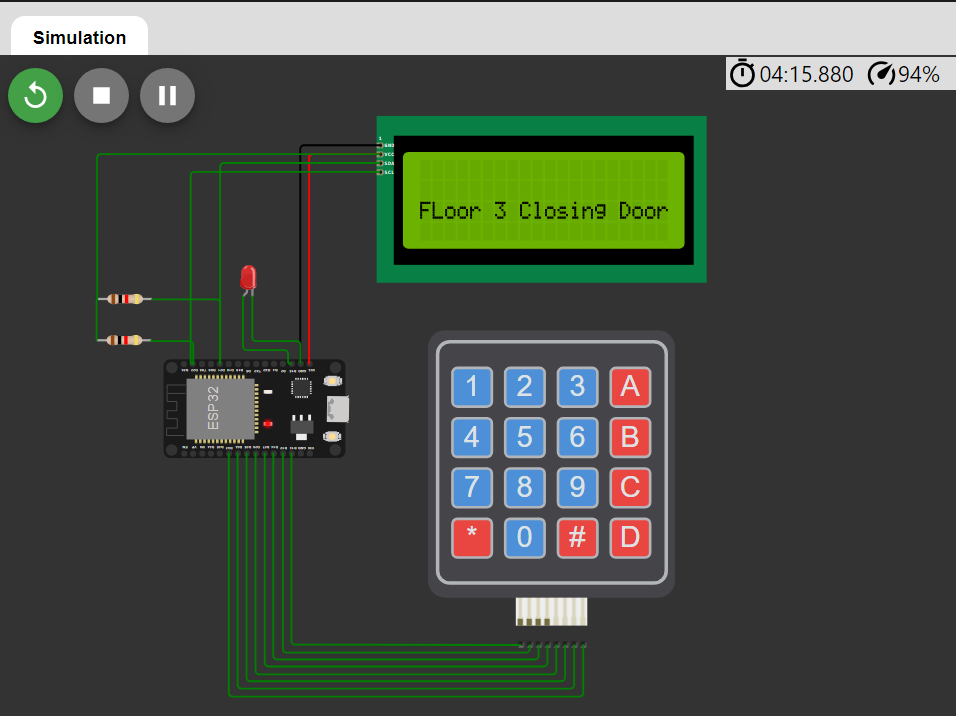
\includegraphics[width=0.5\textwidth]{img/circuit.png} % Replace example-image with the filename of your image
  \caption{Full circuit}
\end{figure}
\subsection{Screenshots during operation}
% \begin{itemize}
% \item
\begin{figure}[htbp] % Here htbp stands for "here, top, bottom, page"
  \centering
  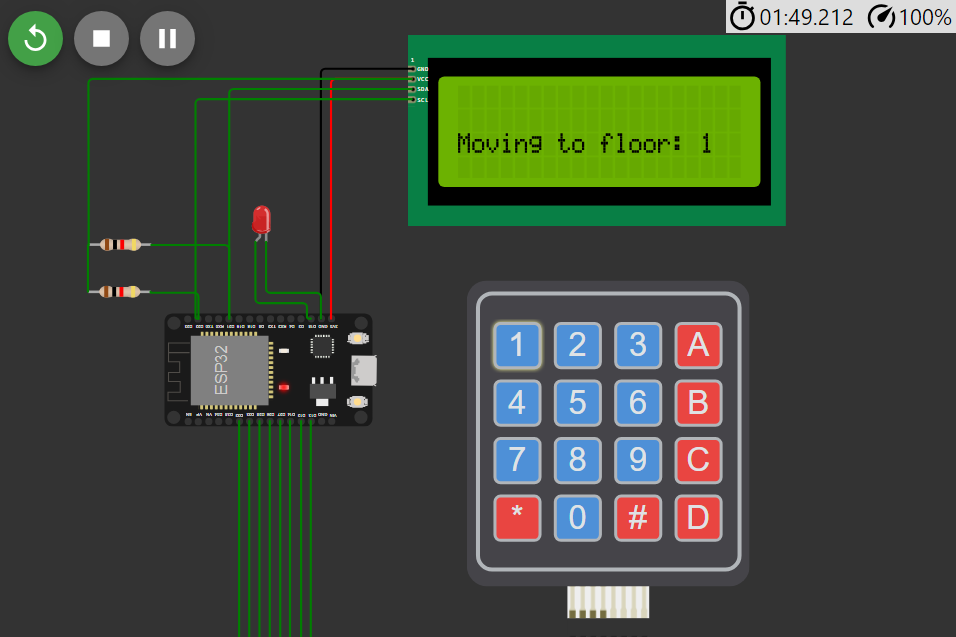
\includegraphics[width=0.5\textwidth]{img/1_move.png} % Replace example-image with the filename of your image
  \caption{Moving to floor 1}
\end{figure}

% \item
\begin{figure}[htbp] % Here htbp stands for "here, top, bottom, page"
  \centering
  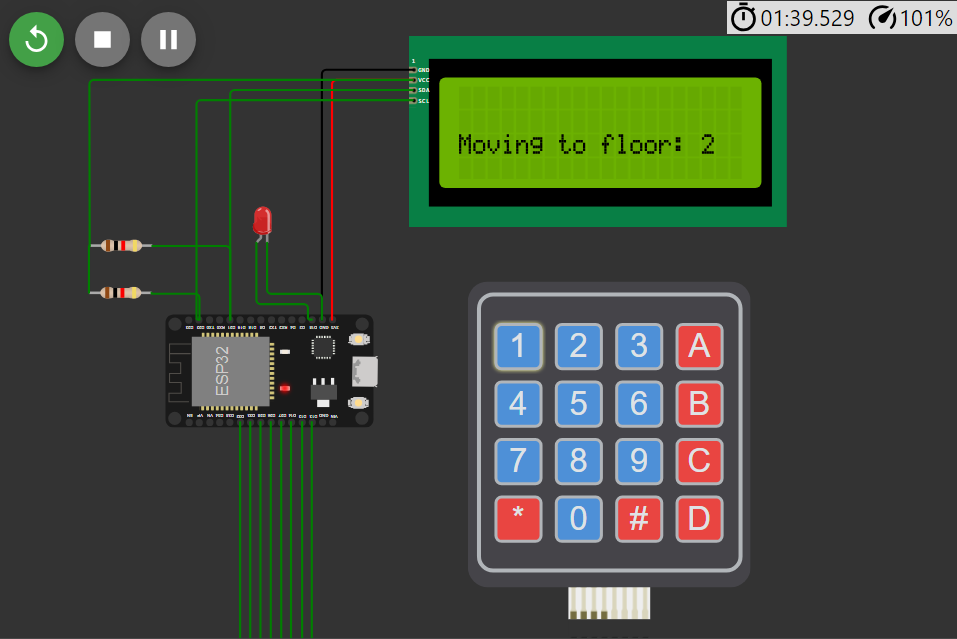
\includegraphics[width=0.5\textwidth]{img/2_move.png} % Replace example-image with the filename of your image
  \caption{Moving to floor 2}
\end{figure}

% \item
\begin{figure}[htbp] % Here htbp stands for "here, top, bottom, page"
  \centering
  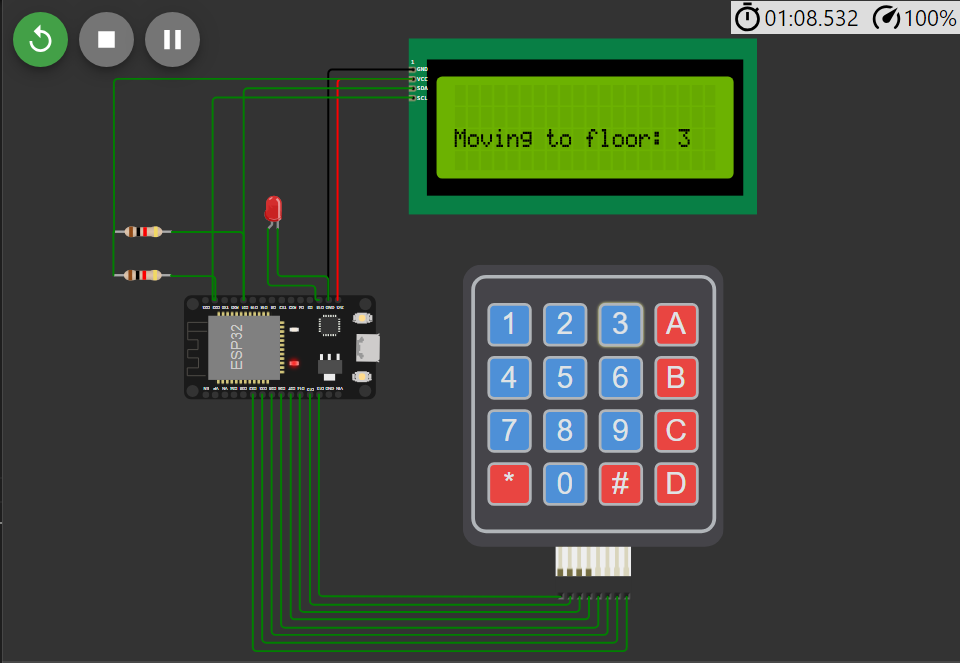
\includegraphics[width=0.5\textwidth]{img/3_move.png} % Replace example-image with the filename of your image
  \caption{Moving to floor 3}
\end{figure}


% \item
\begin{figure}[!htbp] % Here htbp stands for "here, top, bottom, page"
  \centering

  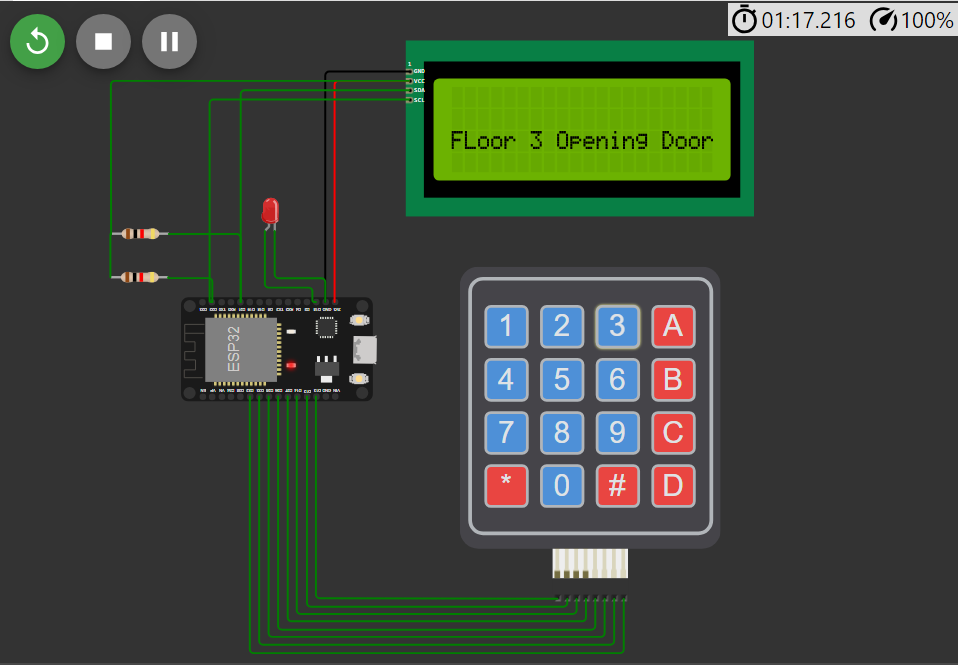
\includegraphics[width=0.45\textwidth]{img/3_open.png} % Replace example-image with the filename of your image
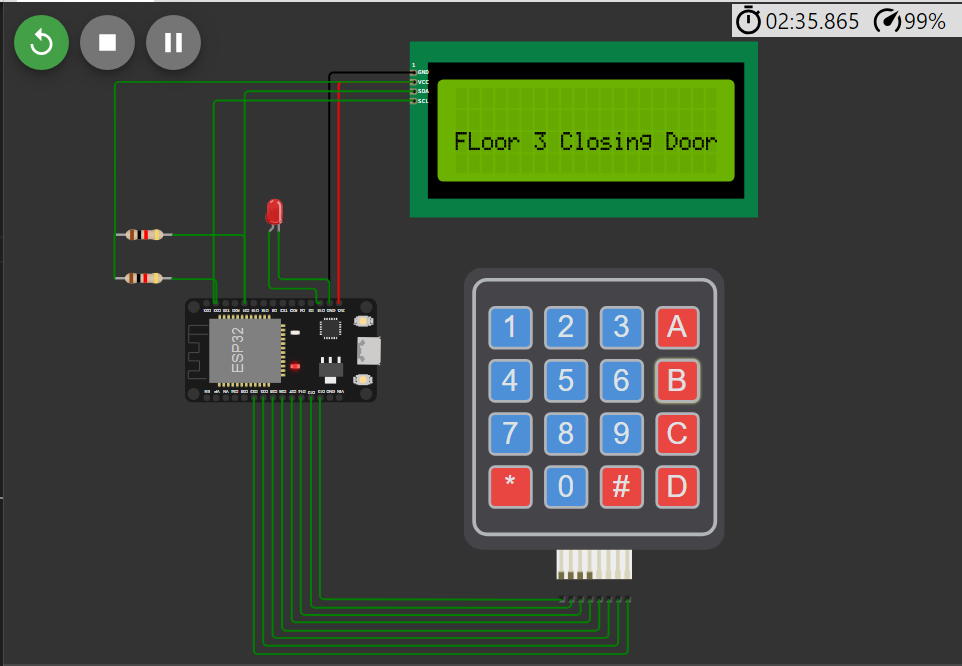
\includegraphics[width=0.45\textwidth]{img/3_close.png}
  \caption{Opening and closing lift doors}
\end{figure}


\begin{figure}[!htbp] % Here htbp stands for "here, top, bottom, page"
  \centering

  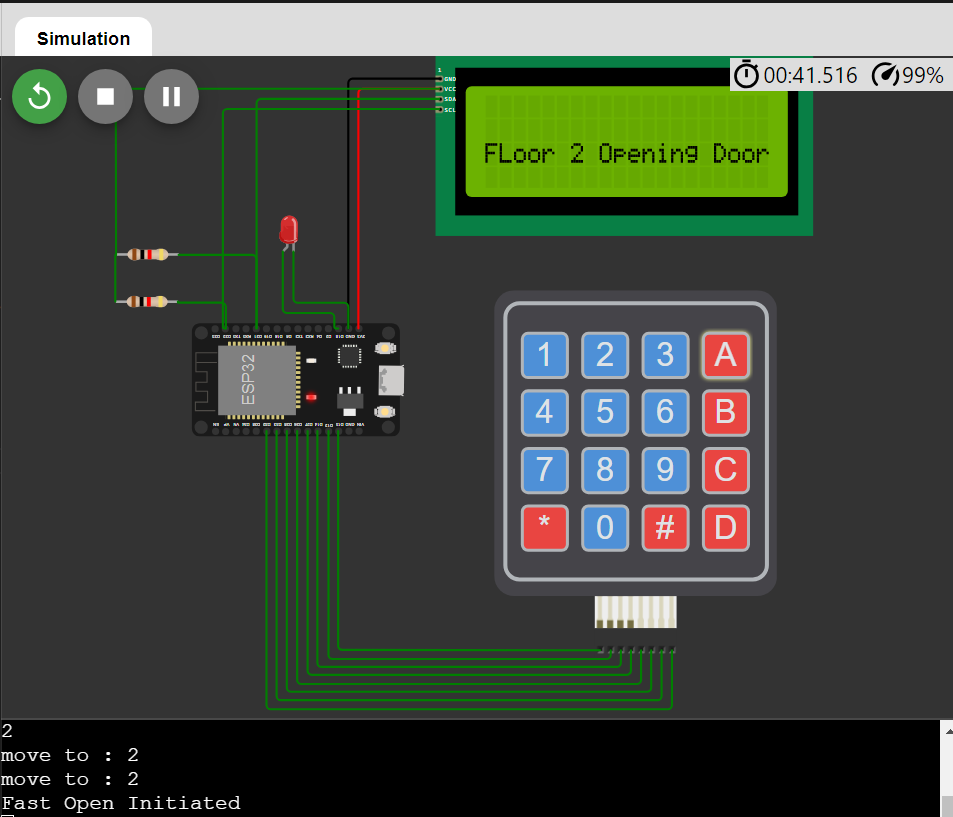
\includegraphics[width=0.45\textwidth]{img/fast_open.png}
  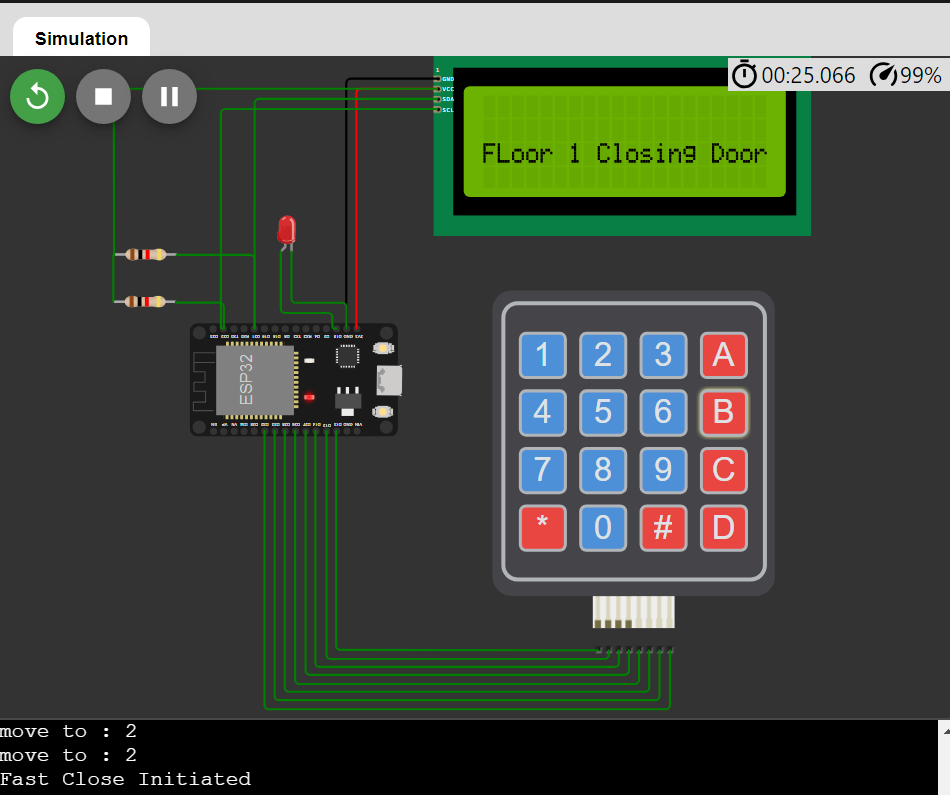
\includegraphics[width=0.45\textwidth]{img/fast_open_close_new.png} % 
  \caption{Fast open (key 'A') and Fast close (key 'B')}
\end{figure}


\begin{figure}[!htbp] % Here htbp stands for "here, top, bottom, page"
  \centering

  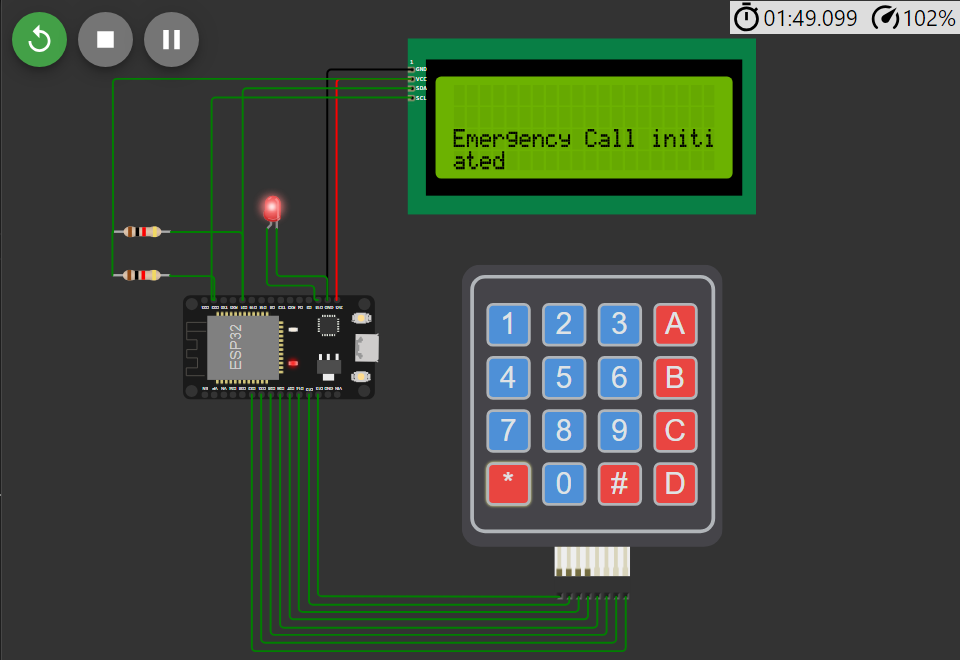
\includegraphics[width=0.45\textwidth]{img/call.png} % 
  \caption{Emergency call and the glowing LED (key '*')}
\end{figure}

\begin{figure}[!htbp] % Here htbp stands for "here, top, bottom, page"
  \centering

  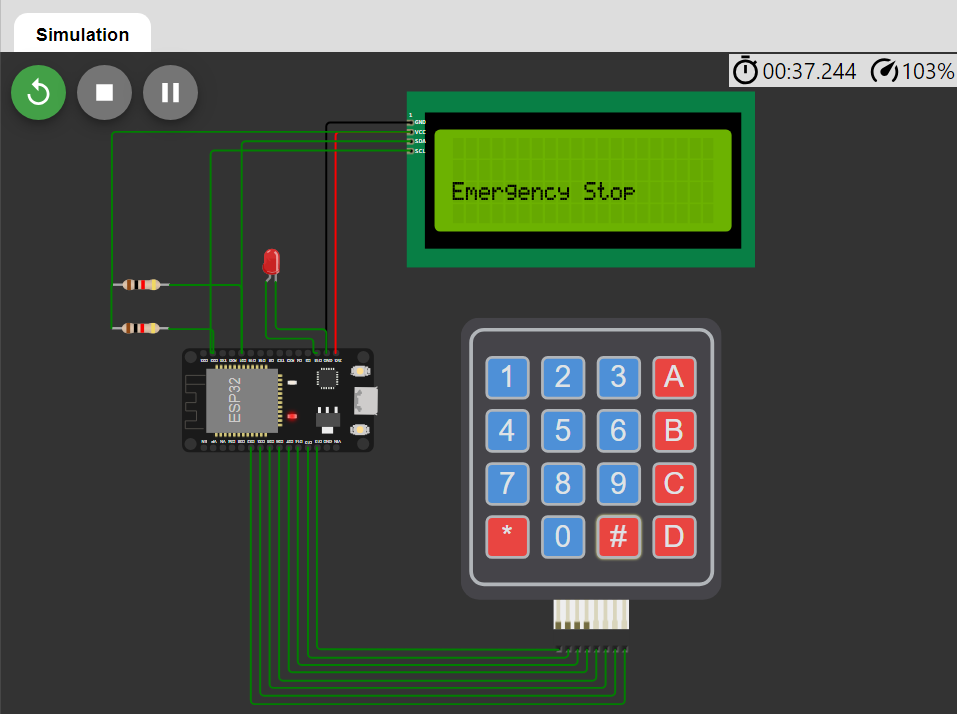
\includegraphics[width=0.45\textwidth]{img/stop.png} % 
  \caption{Emergency stop (key '\#')}
\end{figure}



\clearpage
\section{Possible improvements}
\begin{enumerate}
    \item \textbf{Deselect Option} The lift could have a deselect option such that if a person selects the wrong button, he has the option to deselect it and select the correct one.\\ In a case if the lift has started moving, and then the button is deselected, the lift will move in the same direction, stop on the nearest floor and then continue moving according to the remaining selected buttons.
    \item \textbf{Outer lift control panel} The lift setup may include an external control panel for calling the lift.
    \item \textbf{Non-Stop setting} The lift control panel may have a non-stop setting for a case in which the lift is needed to operate from the ground floor directly to the third and subsequent floor (i.e. it doesn't stop in between the ground floor to the third floor)
\end{enumerate}
% \section{Limitations}
\section{Conclusion}
The Lift Controller Project is all about creating a system that makes elevators in buildings work smoothly and safely. We've put together different parts like the controller, keypad, lights, and screen to make it easy for people to use and to alert for emergencies. 

The system follows a plan for how long things take, like moving between floors or opening and closing doors. This helps everything run smoothly and keeps people moving comfortably. Also, we've added features like quick door buttons and an emergency call button to make it even better.

To summarize, while our current lift controller meets basic requirements, further enhancements are necessary to optimize functionality, efficiency, and safety. These improvements will create a more sophisticated and reliable lift system that meets modern user expectations.


\clearpage

\section*{}
\addcontentsline{toc}{section}{\protect\numberline{}Glossary}
\printglossary[type=\acronymtype]

\clearpage

% \printindex
\clearpage

\begin{appendix}
\section{Appendix 1: Document Statistics}

\begin{itemize}
\item Word Count: 4430
\item Number of Sentences: 380
\item Number of Characters: 24963
\end{itemize}

\section{Appendix 2: Readability Indices}

\begin{itemize}
\item \textbf{Readability Index\footnote{The readability index indicates the approximate reading grade level of a text based on the US education system. The formula takes into account characters in a given word and the words in a given sentence. It varies from 0 - 16+.}:} 1.4

\\This means that this text can be understood by children who can read books with chapters.

\item \textbf{Gunning-Fog Index\footnote{On a scale from 0 -20, the Gunning-Fog Index is a weighted average of the number of words per sentence and the number of long words per word. This can be understood as the text can be understood by someone who left full-time education at a later age than the index. Hence a lower Gunning-Fog index is easier to read.}:} 7.4

\\This means that the text can be easily understood by someone who has passed grade 8, US education standards.

\item \textbf{Flesch Reading Ease\footnote{The Flesch Reading Ease indicates the approximate reading grade level of a text. The formula takes into account sentence length and word length. It is based on a 0-100 scale. A high score means that the text is easier to read.}:} 87 \\This means that this text can be understood by 12-13 year olds.

\item \textbf{Coleman Liau Index\footnote{On a scale of 0 - 17+, the Coleman Liau Index relies on characters and calculates the index based on the number of characters in a word and the number of words in a sentence. The score of the text indicates the US school level a person needs to understand the text.}:} 5.6

\\This means that the text can be easily understood by someone who has passed grade 10, US education standards.

\end{itemize}

\end{appendix}

\clearpage


\end{document}
